\documentclass[aspectratio=169,14pt]{beamer}
\usepackage{iftex}
% xelatex/lualatex: Fira Sans, else Noto Sans. pdflatex fallback (no fontspec needed): TeX Gyre Heros.
\ifPDFTeX
  \usepackage[T1]{fontenc}\usepackage{textcomp}
  \usepackage{tgheros}\renewcommand{\familydefault}{\sfdefault}
\else
  \usepackage{fontspec}
  \IfFontExistsTF{Fira Sans}{}{%
    \setsansfont{Noto Sans}[Ligatures=TeX]\setmainfont{Noto Sans}[Ligatures=TeX]}
\fi
\usetheme[progressbar=frametitle,numbering=none,block=fill]{metropolis}
\ifPDFTeX\else\IfFontExistsTF{Fira Sans}{}{\setsansfont{Noto Sans}\setmainfont{Noto Sans}}\fi
\usepackage{tikz}
\usetikzlibrary{arrows.meta,positioning,shapes.geometric,calc}
\usepackage{qrcode}
\usepackage{xcolor}
% Colours follow the web app tokens in diseno/ui-design.md section 2.1 (Helmut, 2026-10-29).
\date{}
\definecolor{cardano}{HTML}{0066CC}
\definecolor{cardanolight}{HTML}{F5F5F7}
\definecolor{warm}{HTML}{0066CC}
\definecolor{ink}{HTML}{1D1D1F}
\definecolor{paper}{HTML}{FFFFFF}
\definecolor{okgreen}{HTML}{1B7A31}
\definecolor{nogo}{HTML}{B3261E}
\setbeamercolor{normal text}{fg=ink,bg=paper}
\setbeamercolor{alerted text}{fg=warm}
\setbeamercolor{frametitle}{bg=paper,fg=ink}
\setbeamercolor{progress bar}{fg=warm,bg=cardanolight}
\setbeamercolor{title separator}{fg=warm}
\setbeamercolor{block title}{bg=cardano,fg=white}
\setbeamercolor{block body}{bg=cardanolight,fg=ink}
\newcommand{\ph}[1]{\colorbox{warm!25}{\textcolor{nogo}{\texttt{[#1]}}}}
\newcommand{\todo}[1]{\ph{TODO: #1}}
\newcommand{\hero}[1]{{\fontsize{26}{30}\selectfont\bfseries #1}}
\setbeamerfont{subtitle}{size=\normalsize}
% All changeable facts live here. One-line edits.
\newcommand{\TeamName}{Shelfie}
\newcommand{\Tagline}{Paid only when the photo is true.}
\newcommand{\Event}{TUM Blockchain Hackathon 2026 \,\textbullet\, Cardano track}
\newcommand{\City}{Munich}
% MVP job = one store, one photo (N=1, K=1; diseno/decisions.md ADR-16). No store-count macros; multi-store is roadmap.
\newcommand{\PersonaName}{Katharina}
\newcommand{\PersonaInitial}{K}
\newcommand{\PersonaRole}{Field-sales manager, Isarquell (Bavarian craft lemonade)}
% Figures: market numbers sourced in pitch/market-pricing.md (\ph = still unsourced). Prices on slides are illustrative product pricing in EUR, never preprod test amounts (1 tADA per check, 3 tADA per payout).
\newcommand{\CostPerVisit}{€50+}% German Testkauf, mystery.agency / mystery-shopping.de; US audit visit $30-45 (T-ROC 2026)
\newcommand{\LeadTimeDays}{\ph{X days}}
\newcommand{\WasteShare}{\ph{XX\%}}
\newcommand{\PricePerStore}{€12}% pay-as-you-go, illustrative
\newcommand{\PayoutPerTask}{€3.50}% illustrative
\newcommand{\VerifierFee}{< €0.10}% estimate
\newcommand{\GrossMargin}{$\sim$65\%}% (12 - 3.50 - 0.10 - 0.60 escrow) / 12, estimate
\newcommand{\TimeToReport}{\ph{XX min}}
% On-chain proof (Cardano preprod)
\newcommand{\TxLock}{\ph{tx: lock}}
\newcommand{\TxPayout}{\ph{tx: payout}}
\newcommand{\TxSettle}{\ph{tx: settle}}
\newcommand{\UrlLock}{https://preprod.cardanoscan.io/transaction/TODO}
\newcommand{\UrlPayout}{https://preprod.cardanoscan.io/transaction/TODO}
\newcommand{\UrlSettle}{https://preprod.cardanoscan.io/transaction/TODO}
\newcommand{\UrlRepo}{https://github.com/TODO/shelfie}
% Team (roles TBD)
\newcommand{\MemberA}{Helmut}\newcommand{\RoleA}{\ph{A: shell}}
\newcommand{\MemberB}{Isabel}\newcommand{\RoleB}{\ph{B: pay}}
\newcommand{\MemberC}{Fernando}\newcommand{\RoleC}{\ph{C: verifier}}
\newcommand{\MemberD}{Lorenz}\newcommand{\RoleD}{\ph{D: web}}
\newcommand{\ClosingLine}{Agents hire people to look, and the blockchain pays the bill.}

\title{\TeamName}
\subtitle{\Tagline}
\author{\MemberA \,\textbullet\, \MemberB \,\textbullet\, \MemberC \,\textbullet\, \MemberD}
\institute{\Event}
\begin{document}
% Title: shown before the timer starts. Live deck (pitch/live-pitch.md run of show, review/pitch-jury-2026-10-30.md):
% hook, flow, demo, receipts, today/next, close.
{\vfuzz=25pt \setbeamercolor{background canvas}{bg=cardano}\setbeamercolor{normal text}{fg=white,bg=cardano}\setbeamercolor{title separator}{fg=white}
\begin{frame}[plain]
  \titlepage
\end{frame}
}

\begin{frame}[plain]
  \vspace{1em}
  \centering
  
\begin{tikzpicture}
    \fill[cardanolight] (0,0) rectangle (9,2.6);
    \foreach \i in {0,1,2,3,4,5,6,7} {\fill[cardano!70] (0.3+1.05*\i,0.3) rectangle ++(0.7,1.0);
      \fill[cardano!40] (0.3+1.05*\i,1.5) rectangle ++(0.7,0.8);}
    \fill[warm] (4.35,0.3) rectangle ++(0.7,1.0);
    \fill[white,draw=ink] (4.1,-0.4) rectangle ++(1.2,0.4);
    \node[ink] at (4.7,-0.2) {\ph{€?.??}};
  \end{tikzpicture}\\[0.8em]
  \hero{Is our product on this shelf?\\ At what price?}\\[0.6em]
  {\large Right now. In this store.}
\end{frame}

\begin{frame}{\TeamName: \Tagline}
  \centering\vspace{1.5em}
  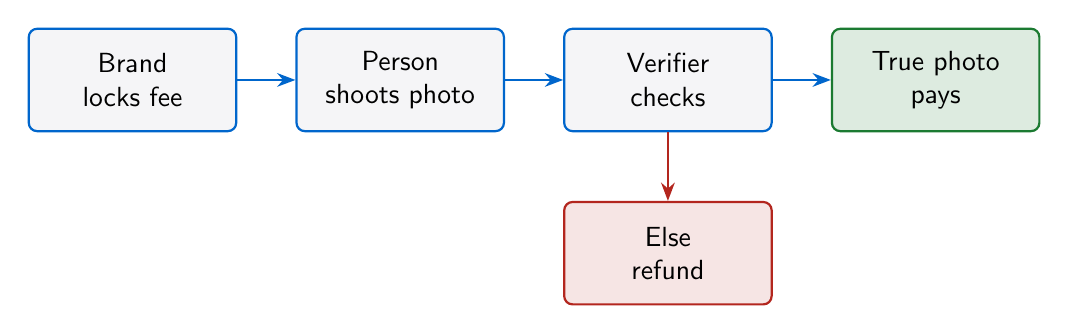
\begin{tikzpicture}[font=\normalsize,
      flowbox/.style={draw=cardano,fill=cardanolight,rounded corners=3pt,thick,minimum height=13mm,text width=24mm,align=center},
      arr/.style={-{Stealth},thick,cardano}]
    \node[flowbox] (a) at (0,0) {Brand\\locks fee};
    \node[flowbox] (b) at (3.4,0) {Person\\shoots photo};
    \node[flowbox] (c) at (6.8,0) {Verifier\\checks};
    \node[flowbox,draw=okgreen,fill=okgreen!15] (d) at (10.2,0) {True photo\\pays};
    \node[flowbox,draw=nogo,fill=nogo!12] (e) at (6.8,-2.2) {Else\\refund};
    \draw[arr] (a)--(b); \draw[arr] (b)--(c); \draw[arr] (c)--(d);
    \draw[arr,nogo] (c)--(e);
  \end{tikzpicture}\\[1.2em]
  {\large For brands entering a market without a field team.}
\end{frame}

{\setbeamercolor{background canvas}{bg=cardano}
\begin{frame}[plain]
  \centering\vspace{3em}
  {\fontsize{60}{66}\selectfont\bfseries\color{white}LIVE DEMO}\\[1em]
  {\Large\color{white!80} Shoot. Verify. Get paid.}
\end{frame}
}

% Live slide 4. Hashes and URLs in facts.tex; fill from codigo/docs/evidence/tx-hashes.md, never from memory.
\begin{frame}{Every step is a receipt on Cardano}
  \centering\scriptsize
  \begin{columns}[T]
    \begin{column}{0.19\textwidth}\centering
      {\bfseries Lock}\\{\color{cardano}earlier run}\\[0.3em]\qrcode[height=1.6cm]{\UrlLock}\\[0.2em]\TxLock
    \end{column}
    \begin{column}{0.19\textwidth}\centering
      {\bfseries Verifier fee}\\{\color{okgreen}live, x402}\\[0.3em]\qrcode[height=1.6cm]{\UrlFee}\\[0.2em]\TxFee
    \end{column}
    \begin{column}{0.19\textwidth}\centering
      {\bfseries Payout}\\{\color{okgreen}live}\\[0.3em]\qrcode[height=1.6cm]{\UrlPayout}\\[0.2em]\TxPayout
    \end{column}
    \begin{column}{0.19\textwidth}\centering
      {\bfseries Settle}\\{\color{cardano}earlier run}\\[0.3em]\qrcode[height=1.6cm]{\UrlSettle}\\[0.2em]\TxSettle
    \end{column}
    \begin{column}{0.19\textwidth}\centering
      {\bfseries Refund}\\{\color{cardano}earlier run}\\[0.3em]\qrcode[height=1.6cm]{\UrlRefund}\\[0.2em]\TxRefund
    \end{column}
  \end{columns}
  \vspace{1em}
  {\small No true photo, no payment: Masumi escrow refunds automatically.\\
  The verifier is a URL the brand can swap.}\\[0.4em]
  Cardano preprod. Scan to open in the explorer.
\end{frame}

% Live slide 5. Market figure checked at source (pitch-plan.md section 4).
\begin{frame}{Today and next}
  \begin{columns}[T]
    \begin{column}{0.42\textwidth}\centering
      {\fontsize{28}{32}\selectfont\bfseries\color{cardano}\MarketServices}\\[0.1em]
      {\scriptsize spent on in-store merchandising per year}\\[0.8em]
      {\fontsize{22}{26}\selectfont\bfseries\color{cardano}\PricePerStore}\\[0.1em]
      {\scriptsize per check, vs \CostPerVisit\ per test purchase}
    \end{column}
    \begin{column}{0.58\textwidth}\small
      \alert{Today}\\
      One shelf, \City, preprod\\
      One real request, no interviews yet\\
      The sign stops stale photos, not the wrong shop\\[0.6em]
      \alert{Next}\\
      Store QR codes prove the location
    \end{column}
  \end{columns}
  \vfill
  {\centering\tiny Beroe (2023 est.). Shelfie price illustrative; test purchase from German agency price lists.\par}
\end{frame}

{\setbeamercolor{background canvas}{bg=cardano}
\begin{frame}[plain]
  \centering\vspace{4em}
  {\fontsize{30}{36}\selectfont\bfseries\color{white}\ClosingLine}\\[1.5em]
  {\large\color{warm}\TeamName}
\end{frame}
}

% Backup slides for Q&A, after the close. 03-problem and 08-proof are kept in sections/ but not shown
% (unsourced placeholders; superseded by 08b-receipts).
\appendix
% Backup for the question "what is live, what is mocked?" (qa-prep.md Q19). Update before the Sat 11:00 freeze to what actually ran.
\begin{frame}{What is real today}
  \small
  \begin{columns}[T]
    \begin{column}{0.33\textwidth}
      {\bfseries\color{okgreen} Live on preprod}\\[0.4em]
      Escrow lock (Masumi)\\
      Verifier fee over x402\\
      Payout to the worker\\
      One-time hand sign, verifier gates
    \end{column}
    \begin{column}{0.33\textwidth}
      {\bfseries\color{cardano} From an earlier run}\\[0.4em]
      Escrow settlement\\
      Refund when no photo passes\\[0.4em]
      {\scriptsize Escrow test runs; the cycle takes 30--45 minutes.}
    \end{column}
    \begin{column}{0.33\textwidth}
      {\bfseries\color{nogo} Not built yet}\\[0.4em]
      Location proof (store QR next)\\
      Strangers as workers\\
      Identity checks\\
      Mainnet, real money
    \end{column}
  \end{columns}
  \vspace{1em}
  {\scriptsize Demo: our own printed price tags, teammates as workers, a seeded Munich catalog.}
\end{frame}

\begin{frame}{The market}
  \centering
  \begin{columns}[T]
    \begin{column}{0.33\textwidth}\centering
      {\fontsize{28}{32}\selectfont\bfseries\color{cardano}\MarketPain}\\[0.2em]
      {\small retail sales lost to\\ empty shelves per year}
    \end{column}
    \begin{column}{0.33\textwidth}\centering
      {\fontsize{28}{32}\selectfont\bfseries\color{cardano}\MarketServices}\\[0.2em]
      {\small spent on in-store\\ merchandising per year}
    \end{column}
    \begin{column}{0.33\textwidth}\centering
      {\fontsize{28}{32}\selectfont\bfseries\color{cardano}\MarketMystery}\\[0.2em]
      {\small mystery shopping,\\ paid per visit}
    \end{column}
  \end{columns}
  \vspace{1.2em}
  {\large One check: \alert{\PricePerStore}, vs \CostPerVisit\ per test purchase.}\\[0.6em]
  {\scriptsize \MarketSources\ Shelfie prices are illustrative estimates.}
\end{frame}

\begin{frame}{Why Cardano}
  \begin{columns}[T]
    \begin{column}{0.5\textwidth}
      \alert{Escrow} Masumi holds the fee until delivery\\[0.6em]
      \alert{x402} the verifier is paid per check, no accounts
    \end{column}
    \begin{column}{0.5\textwidth}
      \alert{Cheap fees} micro-payouts to humans make sense\\[0.6em]
      \alert{Receipts} every check, payout and refund is a public tx
    \end{column}
  \end{columns}
\end{frame}

\begin{frame}{The customer}
  \begin{columns}[T]
    \begin{column}{0.4\textwidth}\centering
      
\begin{tikzpicture}
        \fill[cardano] (0,0) circle (1.3);
        \node[white] at (0,0) {\fontsize{34}{34}\selectfont\bfseries \PersonaInitial};
      \end{tikzpicture}
    \end{column}
    \begin{column}{0.6\textwidth}
      {\Large\bfseries \PersonaName}\\[0.3em]
      \PersonaRole\\[1em]
      \alert{Needs today:} on shelf? at what price?\\[0.4em]
      \alert{Has:} an agency, days of lead time, an invoice.\\[0.8em]{\scriptsize Fictional persona.}
    \end{column}
  \end{columns}
\end{frame}

\begin{frame}{How it works}
  \centering
  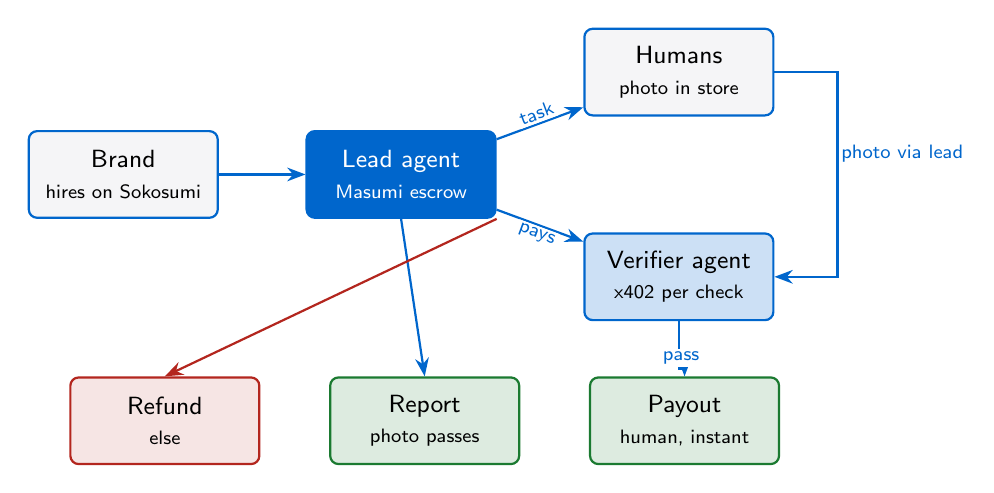
\begin{tikzpicture}[scale=1.0,transform shape,
      node distance=9mm and 11mm, font=\small,
      box/.style={draw=cardano,fill=cardanolight,rounded corners=3pt,thick,minimum height=11mm,minimum width=24mm,align=center},
      hot/.style={box,fill=cardano,text=white},
      warmb/.style={box,draw=warm,fill=warm!20},
      arr/.style={-{Stealth},thick,cardano},
      lab/.style={font=\scriptsize,fill=paper,inner sep=1pt}]
    \node[box] (brand) {Brand\\{\scriptsize hires on Sokosumi}};
    \node[hot,right=of brand] (lead) {Lead agent\\{\scriptsize Masumi escrow}};
    \node[box,right=of lead,yshift=13mm] (human) {Humans\\{\scriptsize photo in store}};
    \node[warmb,right=of lead,yshift=-13mm] (ver) {Verifier agent\\{\scriptsize x402 per check}};
    \node[box,below=20mm of lead,xshift=36mm,draw=okgreen,fill=okgreen!15] (pay) {Payout\\{\scriptsize human, instant}};
    \node[box,below=20mm of lead,xshift=3mm,draw=okgreen,fill=okgreen!15] (rep) {Report\\{\scriptsize photo passes}};
    \node[box,below=20mm of lead,xshift=-30mm,draw=nogo,fill=nogo!12] (ref) {Refund\\{\scriptsize else}};
    \draw[arr] (brand)--(lead);
    \draw[arr] (lead)--node[lab,above,sloped]{task}(human);
    \draw[arr] (human.east) -- ++(8mm,0) |- node[lab,pos=.2,right]{photo via lead}(ver.east);
    \draw[arr] (lead)--node[lab,below,sloped]{pays}(ver);
    \draw[arr] (ver.south)--++(0,-6mm)-|node[lab,pos=.2,above]{pass}(pay.north);
    \draw[arr] (lead.south)--(rep.north);
    \draw[arr,nogo] (lead.south east)--(ref.north);
  \end{tikzpicture}
\end{frame}

\begin{frame}{Three payment gates}
  \begin{columns}[T]
    \begin{column}{0.32\textwidth}\centering
      {\hero{\color{warm}1}}\\[0.4em]{\large\bfseries Photo gate}\\
      One-time hand sign, price and product read, within 90 s.\\[0.4em]
      $\rightarrow$ \alert{pays the human}
    \end{column}
    \begin{column}{0.32\textwidth}\centering
      {\hero{\color{warm}2}}\\[0.4em]{\large\bfseries Job gate}\\
      The passing photo is the job result.\\[0.4em]
      $\rightarrow$ \alert{escrow settles}
    \end{column}
    \begin{column}{0.32\textwidth}\centering
      {\hero{\color{warm}3}}\\[0.4em]{\large\bfseries Fallback}\\
      Otherwise the result is withheld.\\[0.4em]
      $\rightarrow$ \alert{automatic refund}
    \end{column}
  \end{columns}
\end{frame}

\begin{frame}{Business model}
  \centering
  \begin{columns}[T]
    \begin{column}{0.5\textwidth}
      \alert{Brand pays} \PricePerStore\ per verified store\\[0.5em]
      \alert{Human earns} \PayoutPerTask\ per passed task\\[0.5em]
      \alert{Verifier costs} \VerifierFee\ per check
    \end{column}
    \begin{column}{0.5\textwidth}
      \alert{Gross margin} \GrossMargin\\[0.5em]
      \alert{Report in} \TimeToReport\ instead of days\\[0.5em]
      \alert{Failed checks cost the brand} nothing
    \end{column}
  \end{columns}
  \vspace{1em}\todo{unit economics from CFO model}\\[0.4em]{\scriptsize Illustrative product pricing in EUR; not the preprod test amounts.}
\end{frame}

\begin{frame}{Beyond the hackathon}
  \centering
  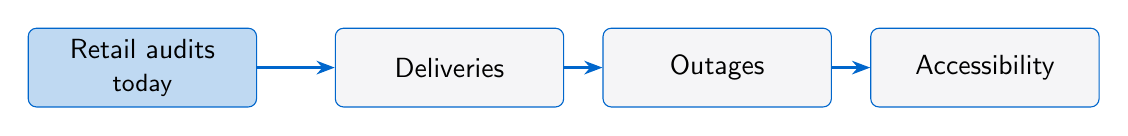
\begin{tikzpicture}[font=\normalsize,
     pack/.style={draw=cardano,fill=cardanolight,rounded corners=3pt,minimum width=2.9cm,minimum height=1cm,align=center}]
    \node[pack,fill=warm!25,draw=warm] (a) at (0,0) {Retail audits\\{\small today}};
    \node[pack] (b) at (3.9,0) {Deliveries};
    \node[pack] (c) at (7.3,0) {Outages};
    \node[pack] (d) at (10.7,0) {Accessibility};
    \draw[-{Stealth},thick,cardano] (a)--(b);\draw[-{Stealth},thick,cardano] (b)--(c);\draw[-{Stealth},thick,cardano] (c)--(d);
  \end{tikzpicture}\\[1.5em]
  {\large AI agents can browse the web, but not see the world.\\[0.2em]
  One engine: any \alert{proof-of-real-world task} is a domain pack.}\\[0.6em]
  {\scriptsize Roadmap; only retail checks are built. Next: store QR codes for location.}
\end{frame}

\begin{frame}{The idea}
  \centering\vspace{1.5em}
  \hero{An agent hires people\\ to photograph shelves.}\\[1em]
  {\Large It pays them \alert{only if the photo is verified true}.}
\end{frame}

\begin{frame}{Team}
  \centering
  \begin{columns}[T]
    \begin{column}{0.24\textwidth}\centering {\large\bfseries\MemberA}\\ \RoleA\end{column}
    \begin{column}{0.24\textwidth}\centering {\large\bfseries\MemberB}\\ \RoleB\end{column}
    \begin{column}{0.24\textwidth}\centering {\large\bfseries\MemberC}\\ \RoleC\end{column}
    \begin{column}{0.24\textwidth}\centering {\large\bfseries\MemberD}\\ \RoleD\end{column}
  \end{columns}
\end{frame}

\end{document}
